\documentclass[tikz,border=1mm,10pt]{standalone}
\usetikzlibrary{patterns}
%\usepackage[dvipsnames]{xcolor}
%\usepackage{pgfplots}
%\pgfplotsset{compat=1.5.1}
\begin{document}
	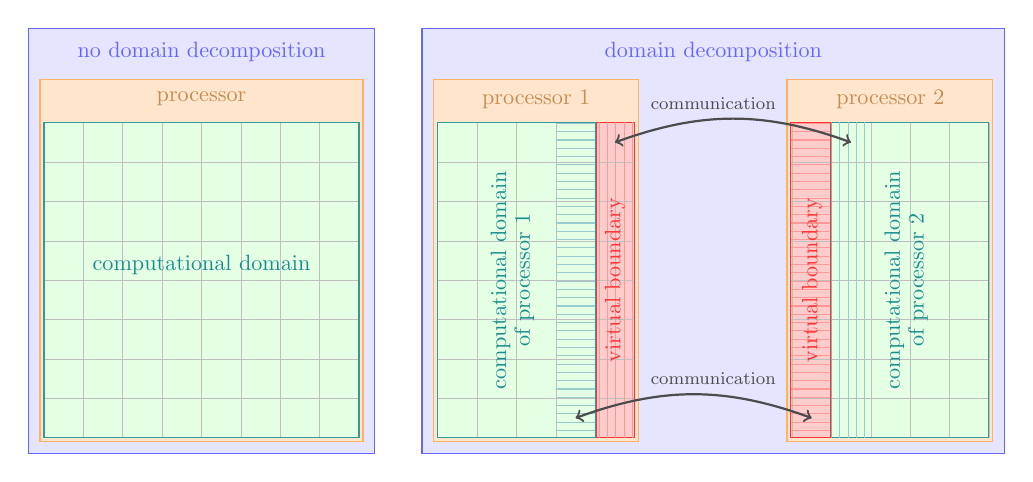
\begin{tikzpicture}[xscale=1,yscale=1,samples=400, transform shape,every node/.style={scale=.8}]
%===============
%	Sequential
%===============
	%Outer rect
	\filldraw[fill=blue!10,draw=blue!60,line width=.15mm] (-1.2,-1.2) rectangle (3.2,4.2);
	\filldraw[fill=orange!20,draw=orange!60,line width=.15mm] (-1.05,-1.05) rectangle (3.05,3.55);
	
	%Grid
	\filldraw[fill=green!10,draw=teal!80, line width=.15mm] (-1,-1) rectangle (3,3);
	\draw[step=0.5cm,lightgray,very thin] (-1,-1) grid (3,3);
	\draw[draw=teal!80, line width=.15mm] (-1,-1) rectangle (3,3);

	%Text
	\node[blue!60] at (1, 3.9) {no domain decomposition};
	\node[teal!90] at (1, 1.2) {computational domain};
	\node[brown!90] at (1, 3.3) {processor};


%===============
%	Parallel
%===============
	%Outer rect
	\filldraw[fill=blue!10,draw=blue!60,line width=.15mm] (3.8,-1.2) rectangle (11.2,4.2);
	\filldraw[fill=orange!20,draw=orange!60,line width=.15mm] (3.95,-1.05) rectangle (6.55,3.55);	
	\filldraw[fill=orange!20,draw=orange!60,line width=.15mm] (8.435,-1.05) rectangle (11.05,3.55);
	
	
	%Grid left
	\filldraw[fill=green!10,draw=teal!80, line width=.15mm] (4,-1) rectangle (6,3);
	\draw[step=0.5cm,lightgray,very thin] (4,-1) grid (6,3);
	\draw[draw=teal!80, line width=.15mm] (4,-1) rectangle (6,3);
	\fill[pattern=horizontal lines, pattern color=teal!40]  (5.5,-1) rectangle (6,3);
	
	%virtual left
	\filldraw[fill=red!20,draw=red!80, line width=.15mm] (6.015,-1) rectangle (6.5,3);
	\draw[step=0.5cm,lightgray,very thin] (6.015,-1) grid (6.5,3);
	\draw[draw=red!80, line width=.15mm] (6.015,-1) rectangle (6.5,3);
	\fill[pattern=vertical lines, pattern color=red!40]  (6.015,-1) rectangle (6.5,3);
		
	%Grid right
	\filldraw[fill=green!10,draw=teal!80, line width=.15mm] (9,-1) rectangle (11,3);
	\draw[step=0.5cm,lightgray,very thin] (9,-1) grid (11,3);
	\draw[draw=teal!80, line width=.15mm] (9,-1) rectangle (11,3);
	\fill[pattern=vertical lines, pattern color=teal!40] (9.0,-1) rectangle (9.5,3);
	
	%virtual right
	\filldraw[fill=red!20,draw=red!80, line width=.15mm] (8.485,-1) rectangle (8.985,3);
	\draw[step=0.5cm,lightgray,very thin] (8.485,-1) grid (8.985,3);
	\draw[draw=red!80, line width=.15mm] (8.485,-1) rectangle (8.985,3);
	\fill[pattern=horizontal lines, pattern color=red!40]  (8.485,-1) rectangle (8.985,3);
	
	
	
	%Text
	\node[blue!60] at (7.5, 3.9) {domain decomposition};
	\node[brown!90] at (5.25, 3.3) {processor 1};
	\node[brown!90] at (9.75, 3.3) {processor 2};
	
	\node[rotate=90, teal!90] at (4.8, 1) {computational domain};
	\node[rotate=90, teal!90] at (5.1, 1) {of processor 1};
	
	\node[rotate=90, teal!90] at (9.8, 1) {computational domain};
	\node[rotate=90, teal!90] at (10.1, 1) {of processor 2};
	
	\node[rotate=90, red!80] at (6.25, 1) {virtual boundary};
	\node[rotate=90, red!80] at (8.75, 1) {virtual boundary};
	
	\node[black!70] at (7.5, 3.25) {\footnotesize communication};
	\node[black!70] at (7.5, -0.25) {\footnotesize communication};

	%Arrows
	\draw[<->, black!70, thick] (5.75,-0.75) to[bend right=-20]
	node[above] {} (8.75,-0.75);
	\draw[<->, black!70, thick] (6.25,2.75) to[bend right=-20] (9.25,2.75);

	\end{tikzpicture}
\end{document}